\documentclass[11pt]{article}

    
    
    \usepackage[T1]{fontenc}
    % Nicer default font (+ math font) than Computer Modern for most use cases
    \usepackage{mathpazo}

    % Basic figure setup, for now with no caption control since it's done
    % automatically by Pandoc (which extracts ![](path) syntax from Markdown).
    \usepackage{graphicx}
    % We will generate all images so they have a width \maxwidth. This means
    % that they will get their normal width if they fit onto the page, but
    % are scaled down if they would overflow the margins.
    \makeatletter
    \def\maxwidth{\ifdim\Gin@nat@width>\linewidth\linewidth
    \else\Gin@nat@width\fi}
    \makeatother
    \let\Oldincludegraphics\includegraphics
    % Set max figure width to be 80% of text width, for now hardcoded.
    \renewcommand{\includegraphics}[1]{\Oldincludegraphics[width=.8\maxwidth]{#1}}
    % Ensure that by default, figures have no caption (until we provide a
    % proper Figure object with a Caption API and a way to capture that
    % in the conversion process - todo).
    \usepackage{caption}
    \DeclareCaptionLabelFormat{nolabel}{}
    \captionsetup{labelformat=nolabel}

    \usepackage{adjustbox} % Used to constrain images to a maximum size 
    \usepackage{xcolor} % Allow colors to be defined
    \usepackage{enumerate} % Needed for markdown enumerations to work
    \usepackage{geometry} % Used to adjust the document margins
    \usepackage{amsmath} % Equations
    \usepackage{amssymb} % Equations
    \usepackage{textcomp} % defines textquotesingle
    % Hack from http://tex.stackexchange.com/a/47451/13684:
    \AtBeginDocument{%
        \def\PYZsq{\textquotesingle}% Upright quotes in Pygmentized code
    }
    \usepackage{upquote} % Upright quotes for verbatim code
    \usepackage{eurosym} % defines \euro
    \usepackage[mathletters]{ucs} % Extended unicode (utf-8) support
    \usepackage[utf8x]{inputenc} % Allow utf-8 characters in the tex document
    \usepackage{fancyvrb} % verbatim replacement that allows latex
    \usepackage{grffile} % extends the file name processing of package graphics 
                         % to support a larger range 
    % The hyperref package gives us a pdf with properly built
    % internal navigation ('pdf bookmarks' for the table of contents,
    % internal cross-reference links, web links for URLs, etc.)
    \usepackage{hyperref}
    \usepackage{longtable} % longtable support required by pandoc >1.10
    \usepackage{booktabs}  % table support for pandoc > 1.12.2
    \usepackage[inline]{enumitem} % IRkernel/repr support (it uses the enumerate* environment)
    \usepackage[normalem]{ulem} % ulem is needed to support strikethroughs (\sout)
                                % normalem makes italics be italics, not underlines
    

    
    
    % Colors for the hyperref package
    \definecolor{urlcolor}{rgb}{0,.145,.698}
    \definecolor{linkcolor}{rgb}{.71,0.21,0.01}
    \definecolor{citecolor}{rgb}{.12,.54,.11}

    % ANSI colors
    \definecolor{ansi-black}{HTML}{3E424D}
    \definecolor{ansi-black-intense}{HTML}{282C36}
    \definecolor{ansi-red}{HTML}{E75C58}
    \definecolor{ansi-red-intense}{HTML}{B22B31}
    \definecolor{ansi-green}{HTML}{00A250}
    \definecolor{ansi-green-intense}{HTML}{007427}
    \definecolor{ansi-yellow}{HTML}{DDB62B}
    \definecolor{ansi-yellow-intense}{HTML}{B27D12}
    \definecolor{ansi-blue}{HTML}{208FFB}
    \definecolor{ansi-blue-intense}{HTML}{0065CA}
    \definecolor{ansi-magenta}{HTML}{D160C4}
    \definecolor{ansi-magenta-intense}{HTML}{A03196}
    \definecolor{ansi-cyan}{HTML}{60C6C8}
    \definecolor{ansi-cyan-intense}{HTML}{258F8F}
    \definecolor{ansi-white}{HTML}{C5C1B4}
    \definecolor{ansi-white-intense}{HTML}{A1A6B2}

    % commands and environments needed by pandoc snippets
    % extracted from the output of `pandoc -s`
    \providecommand{\tightlist}{%
      \setlength{\itemsep}{0pt}\setlength{\parskip}{0pt}}
    \DefineVerbatimEnvironment{Highlighting}{Verbatim}{commandchars=\\\{\}}
    % Add ',fontsize=\small' for more characters per line
    \newenvironment{Shaded}{}{}
    \newcommand{\KeywordTok}[1]{\textcolor[rgb]{0.00,0.44,0.13}{\textbf{{#1}}}}
    \newcommand{\DataTypeTok}[1]{\textcolor[rgb]{0.56,0.13,0.00}{{#1}}}
    \newcommand{\DecValTok}[1]{\textcolor[rgb]{0.25,0.63,0.44}{{#1}}}
    \newcommand{\BaseNTok}[1]{\textcolor[rgb]{0.25,0.63,0.44}{{#1}}}
    \newcommand{\FloatTok}[1]{\textcolor[rgb]{0.25,0.63,0.44}{{#1}}}
    \newcommand{\CharTok}[1]{\textcolor[rgb]{0.25,0.44,0.63}{{#1}}}
    \newcommand{\StringTok}[1]{\textcolor[rgb]{0.25,0.44,0.63}{{#1}}}
    \newcommand{\CommentTok}[1]{\textcolor[rgb]{0.38,0.63,0.69}{\textit{{#1}}}}
    \newcommand{\OtherTok}[1]{\textcolor[rgb]{0.00,0.44,0.13}{{#1}}}
    \newcommand{\AlertTok}[1]{\textcolor[rgb]{1.00,0.00,0.00}{\textbf{{#1}}}}
    \newcommand{\FunctionTok}[1]{\textcolor[rgb]{0.02,0.16,0.49}{{#1}}}
    \newcommand{\RegionMarkerTok}[1]{{#1}}
    \newcommand{\ErrorTok}[1]{\textcolor[rgb]{1.00,0.00,0.00}{\textbf{{#1}}}}
    \newcommand{\NormalTok}[1]{{#1}}
    
    % Additional commands for more recent versions of Pandoc
    \newcommand{\ConstantTok}[1]{\textcolor[rgb]{0.53,0.00,0.00}{{#1}}}
    \newcommand{\SpecialCharTok}[1]{\textcolor[rgb]{0.25,0.44,0.63}{{#1}}}
    \newcommand{\VerbatimStringTok}[1]{\textcolor[rgb]{0.25,0.44,0.63}{{#1}}}
    \newcommand{\SpecialStringTok}[1]{\textcolor[rgb]{0.73,0.40,0.53}{{#1}}}
    \newcommand{\ImportTok}[1]{{#1}}
    \newcommand{\DocumentationTok}[1]{\textcolor[rgb]{0.73,0.13,0.13}{\textit{{#1}}}}
    \newcommand{\AnnotationTok}[1]{\textcolor[rgb]{0.38,0.63,0.69}{\textbf{\textit{{#1}}}}}
    \newcommand{\CommentVarTok}[1]{\textcolor[rgb]{0.38,0.63,0.69}{\textbf{\textit{{#1}}}}}
    \newcommand{\VariableTok}[1]{\textcolor[rgb]{0.10,0.09,0.49}{{#1}}}
    \newcommand{\ControlFlowTok}[1]{\textcolor[rgb]{0.00,0.44,0.13}{\textbf{{#1}}}}
    \newcommand{\OperatorTok}[1]{\textcolor[rgb]{0.40,0.40,0.40}{{#1}}}
    \newcommand{\BuiltInTok}[1]{{#1}}
    \newcommand{\ExtensionTok}[1]{{#1}}
    \newcommand{\PreprocessorTok}[1]{\textcolor[rgb]{0.74,0.48,0.00}{{#1}}}
    \newcommand{\AttributeTok}[1]{\textcolor[rgb]{0.49,0.56,0.16}{{#1}}}
    \newcommand{\InformationTok}[1]{\textcolor[rgb]{0.38,0.63,0.69}{\textbf{\textit{{#1}}}}}
    \newcommand{\WarningTok}[1]{\textcolor[rgb]{0.38,0.63,0.69}{\textbf{\textit{{#1}}}}}
    
    
    % Define a nice break command that doesn't care if a line doesn't already
    % exist.
    \def\br{\hspace*{\fill} \\* }
    % Math Jax compatability definitions
    \def\gt{>}
    \def\lt{<}
    % Document parameters
    \title{Practica1\_Analisis\_Numerico}
    
    
    

    % Pygments definitions
    
\makeatletter
\def\PY@reset{\let\PY@it=\relax \let\PY@bf=\relax%
    \let\PY@ul=\relax \let\PY@tc=\relax%
    \let\PY@bc=\relax \let\PY@ff=\relax}
\def\PY@tok#1{\csname PY@tok@#1\endcsname}
\def\PY@toks#1+{\ifx\relax#1\empty\else%
    \PY@tok{#1}\expandafter\PY@toks\fi}
\def\PY@do#1{\PY@bc{\PY@tc{\PY@ul{%
    \PY@it{\PY@bf{\PY@ff{#1}}}}}}}
\def\PY#1#2{\PY@reset\PY@toks#1+\relax+\PY@do{#2}}

\expandafter\def\csname PY@tok@gd\endcsname{\def\PY@tc##1{\textcolor[rgb]{0.63,0.00,0.00}{##1}}}
\expandafter\def\csname PY@tok@gu\endcsname{\let\PY@bf=\textbf\def\PY@tc##1{\textcolor[rgb]{0.50,0.00,0.50}{##1}}}
\expandafter\def\csname PY@tok@gt\endcsname{\def\PY@tc##1{\textcolor[rgb]{0.00,0.27,0.87}{##1}}}
\expandafter\def\csname PY@tok@gs\endcsname{\let\PY@bf=\textbf}
\expandafter\def\csname PY@tok@gr\endcsname{\def\PY@tc##1{\textcolor[rgb]{1.00,0.00,0.00}{##1}}}
\expandafter\def\csname PY@tok@cm\endcsname{\let\PY@it=\textit\def\PY@tc##1{\textcolor[rgb]{0.25,0.50,0.50}{##1}}}
\expandafter\def\csname PY@tok@vg\endcsname{\def\PY@tc##1{\textcolor[rgb]{0.10,0.09,0.49}{##1}}}
\expandafter\def\csname PY@tok@vi\endcsname{\def\PY@tc##1{\textcolor[rgb]{0.10,0.09,0.49}{##1}}}
\expandafter\def\csname PY@tok@vm\endcsname{\def\PY@tc##1{\textcolor[rgb]{0.10,0.09,0.49}{##1}}}
\expandafter\def\csname PY@tok@mh\endcsname{\def\PY@tc##1{\textcolor[rgb]{0.40,0.40,0.40}{##1}}}
\expandafter\def\csname PY@tok@cs\endcsname{\let\PY@it=\textit\def\PY@tc##1{\textcolor[rgb]{0.25,0.50,0.50}{##1}}}
\expandafter\def\csname PY@tok@ge\endcsname{\let\PY@it=\textit}
\expandafter\def\csname PY@tok@vc\endcsname{\def\PY@tc##1{\textcolor[rgb]{0.10,0.09,0.49}{##1}}}
\expandafter\def\csname PY@tok@il\endcsname{\def\PY@tc##1{\textcolor[rgb]{0.40,0.40,0.40}{##1}}}
\expandafter\def\csname PY@tok@go\endcsname{\def\PY@tc##1{\textcolor[rgb]{0.53,0.53,0.53}{##1}}}
\expandafter\def\csname PY@tok@cp\endcsname{\def\PY@tc##1{\textcolor[rgb]{0.74,0.48,0.00}{##1}}}
\expandafter\def\csname PY@tok@gi\endcsname{\def\PY@tc##1{\textcolor[rgb]{0.00,0.63,0.00}{##1}}}
\expandafter\def\csname PY@tok@gh\endcsname{\let\PY@bf=\textbf\def\PY@tc##1{\textcolor[rgb]{0.00,0.00,0.50}{##1}}}
\expandafter\def\csname PY@tok@ni\endcsname{\let\PY@bf=\textbf\def\PY@tc##1{\textcolor[rgb]{0.60,0.60,0.60}{##1}}}
\expandafter\def\csname PY@tok@nl\endcsname{\def\PY@tc##1{\textcolor[rgb]{0.63,0.63,0.00}{##1}}}
\expandafter\def\csname PY@tok@nn\endcsname{\let\PY@bf=\textbf\def\PY@tc##1{\textcolor[rgb]{0.00,0.00,1.00}{##1}}}
\expandafter\def\csname PY@tok@no\endcsname{\def\PY@tc##1{\textcolor[rgb]{0.53,0.00,0.00}{##1}}}
\expandafter\def\csname PY@tok@na\endcsname{\def\PY@tc##1{\textcolor[rgb]{0.49,0.56,0.16}{##1}}}
\expandafter\def\csname PY@tok@nb\endcsname{\def\PY@tc##1{\textcolor[rgb]{0.00,0.50,0.00}{##1}}}
\expandafter\def\csname PY@tok@nc\endcsname{\let\PY@bf=\textbf\def\PY@tc##1{\textcolor[rgb]{0.00,0.00,1.00}{##1}}}
\expandafter\def\csname PY@tok@nd\endcsname{\def\PY@tc##1{\textcolor[rgb]{0.67,0.13,1.00}{##1}}}
\expandafter\def\csname PY@tok@ne\endcsname{\let\PY@bf=\textbf\def\PY@tc##1{\textcolor[rgb]{0.82,0.25,0.23}{##1}}}
\expandafter\def\csname PY@tok@nf\endcsname{\def\PY@tc##1{\textcolor[rgb]{0.00,0.00,1.00}{##1}}}
\expandafter\def\csname PY@tok@si\endcsname{\let\PY@bf=\textbf\def\PY@tc##1{\textcolor[rgb]{0.73,0.40,0.53}{##1}}}
\expandafter\def\csname PY@tok@s2\endcsname{\def\PY@tc##1{\textcolor[rgb]{0.73,0.13,0.13}{##1}}}
\expandafter\def\csname PY@tok@nt\endcsname{\let\PY@bf=\textbf\def\PY@tc##1{\textcolor[rgb]{0.00,0.50,0.00}{##1}}}
\expandafter\def\csname PY@tok@nv\endcsname{\def\PY@tc##1{\textcolor[rgb]{0.10,0.09,0.49}{##1}}}
\expandafter\def\csname PY@tok@s1\endcsname{\def\PY@tc##1{\textcolor[rgb]{0.73,0.13,0.13}{##1}}}
\expandafter\def\csname PY@tok@dl\endcsname{\def\PY@tc##1{\textcolor[rgb]{0.73,0.13,0.13}{##1}}}
\expandafter\def\csname PY@tok@ch\endcsname{\let\PY@it=\textit\def\PY@tc##1{\textcolor[rgb]{0.25,0.50,0.50}{##1}}}
\expandafter\def\csname PY@tok@m\endcsname{\def\PY@tc##1{\textcolor[rgb]{0.40,0.40,0.40}{##1}}}
\expandafter\def\csname PY@tok@gp\endcsname{\let\PY@bf=\textbf\def\PY@tc##1{\textcolor[rgb]{0.00,0.00,0.50}{##1}}}
\expandafter\def\csname PY@tok@sh\endcsname{\def\PY@tc##1{\textcolor[rgb]{0.73,0.13,0.13}{##1}}}
\expandafter\def\csname PY@tok@ow\endcsname{\let\PY@bf=\textbf\def\PY@tc##1{\textcolor[rgb]{0.67,0.13,1.00}{##1}}}
\expandafter\def\csname PY@tok@sx\endcsname{\def\PY@tc##1{\textcolor[rgb]{0.00,0.50,0.00}{##1}}}
\expandafter\def\csname PY@tok@bp\endcsname{\def\PY@tc##1{\textcolor[rgb]{0.00,0.50,0.00}{##1}}}
\expandafter\def\csname PY@tok@c1\endcsname{\let\PY@it=\textit\def\PY@tc##1{\textcolor[rgb]{0.25,0.50,0.50}{##1}}}
\expandafter\def\csname PY@tok@fm\endcsname{\def\PY@tc##1{\textcolor[rgb]{0.00,0.00,1.00}{##1}}}
\expandafter\def\csname PY@tok@o\endcsname{\def\PY@tc##1{\textcolor[rgb]{0.40,0.40,0.40}{##1}}}
\expandafter\def\csname PY@tok@kc\endcsname{\let\PY@bf=\textbf\def\PY@tc##1{\textcolor[rgb]{0.00,0.50,0.00}{##1}}}
\expandafter\def\csname PY@tok@c\endcsname{\let\PY@it=\textit\def\PY@tc##1{\textcolor[rgb]{0.25,0.50,0.50}{##1}}}
\expandafter\def\csname PY@tok@mf\endcsname{\def\PY@tc##1{\textcolor[rgb]{0.40,0.40,0.40}{##1}}}
\expandafter\def\csname PY@tok@err\endcsname{\def\PY@bc##1{\setlength{\fboxsep}{0pt}\fcolorbox[rgb]{1.00,0.00,0.00}{1,1,1}{\strut ##1}}}
\expandafter\def\csname PY@tok@mb\endcsname{\def\PY@tc##1{\textcolor[rgb]{0.40,0.40,0.40}{##1}}}
\expandafter\def\csname PY@tok@ss\endcsname{\def\PY@tc##1{\textcolor[rgb]{0.10,0.09,0.49}{##1}}}
\expandafter\def\csname PY@tok@sr\endcsname{\def\PY@tc##1{\textcolor[rgb]{0.73,0.40,0.53}{##1}}}
\expandafter\def\csname PY@tok@mo\endcsname{\def\PY@tc##1{\textcolor[rgb]{0.40,0.40,0.40}{##1}}}
\expandafter\def\csname PY@tok@kd\endcsname{\let\PY@bf=\textbf\def\PY@tc##1{\textcolor[rgb]{0.00,0.50,0.00}{##1}}}
\expandafter\def\csname PY@tok@mi\endcsname{\def\PY@tc##1{\textcolor[rgb]{0.40,0.40,0.40}{##1}}}
\expandafter\def\csname PY@tok@kn\endcsname{\let\PY@bf=\textbf\def\PY@tc##1{\textcolor[rgb]{0.00,0.50,0.00}{##1}}}
\expandafter\def\csname PY@tok@cpf\endcsname{\let\PY@it=\textit\def\PY@tc##1{\textcolor[rgb]{0.25,0.50,0.50}{##1}}}
\expandafter\def\csname PY@tok@kr\endcsname{\let\PY@bf=\textbf\def\PY@tc##1{\textcolor[rgb]{0.00,0.50,0.00}{##1}}}
\expandafter\def\csname PY@tok@s\endcsname{\def\PY@tc##1{\textcolor[rgb]{0.73,0.13,0.13}{##1}}}
\expandafter\def\csname PY@tok@kp\endcsname{\def\PY@tc##1{\textcolor[rgb]{0.00,0.50,0.00}{##1}}}
\expandafter\def\csname PY@tok@w\endcsname{\def\PY@tc##1{\textcolor[rgb]{0.73,0.73,0.73}{##1}}}
\expandafter\def\csname PY@tok@kt\endcsname{\def\PY@tc##1{\textcolor[rgb]{0.69,0.00,0.25}{##1}}}
\expandafter\def\csname PY@tok@sc\endcsname{\def\PY@tc##1{\textcolor[rgb]{0.73,0.13,0.13}{##1}}}
\expandafter\def\csname PY@tok@sb\endcsname{\def\PY@tc##1{\textcolor[rgb]{0.73,0.13,0.13}{##1}}}
\expandafter\def\csname PY@tok@sa\endcsname{\def\PY@tc##1{\textcolor[rgb]{0.73,0.13,0.13}{##1}}}
\expandafter\def\csname PY@tok@k\endcsname{\let\PY@bf=\textbf\def\PY@tc##1{\textcolor[rgb]{0.00,0.50,0.00}{##1}}}
\expandafter\def\csname PY@tok@se\endcsname{\let\PY@bf=\textbf\def\PY@tc##1{\textcolor[rgb]{0.73,0.40,0.13}{##1}}}
\expandafter\def\csname PY@tok@sd\endcsname{\let\PY@it=\textit\def\PY@tc##1{\textcolor[rgb]{0.73,0.13,0.13}{##1}}}

\def\PYZbs{\char`\\}
\def\PYZus{\char`\_}
\def\PYZob{\char`\{}
\def\PYZcb{\char`\}}
\def\PYZca{\char`\^}
\def\PYZam{\char`\&}
\def\PYZlt{\char`\<}
\def\PYZgt{\char`\>}
\def\PYZsh{\char`\#}
\def\PYZpc{\char`\%}
\def\PYZdl{\char`\$}
\def\PYZhy{\char`\-}
\def\PYZsq{\char`\'}
\def\PYZdq{\char`\"}
\def\PYZti{\char`\~}
% for compatibility with earlier versions
\def\PYZat{@}
\def\PYZlb{[}
\def\PYZrb{]}
\makeatother


    % Exact colors from NB
    \definecolor{incolor}{rgb}{0.0, 0.0, 0.5}
    \definecolor{outcolor}{rgb}{0.545, 0.0, 0.0}



    
    % Prevent overflowing lines due to hard-to-break entities
    \sloppy 
    % Setup hyperref package
    \hypersetup{
      breaklinks=true,  % so long urls are correctly broken across lines
      colorlinks=true,
      urlcolor=urlcolor,
      linkcolor=linkcolor,
      citecolor=citecolor,
      }
    % Slightly bigger margins than the latex defaults
    
    \geometry{verbose,tmargin=1in,bmargin=1in,lmargin=1in,rmargin=1in}
    
    

    \begin{document}
    
    
    \maketitle
    
    

    
    \section{Parte de Aritmética de Punto
Flotante}\label{parte-de-aritmuxe9tica-de-punto-flotante}

    \subsection{Ejercicio 1 (1 punto)}\label{ejercicio-1}
 La aproximación de Stirling
\[S_n=\sqrt{2\pi n}\cdot\left(\dfrac{n}{\exp(1)}\right)^n\] se usa para
aproximar el factorial \(n!\). \\
Escriba un programa que muestre a modo de tabla tanto a \(n!\) como a
\(S_n\), así como los errores relativos y absolutos para
\(n=1,\dots,20\) 

    \begin{quote}
\begin{itemize}
\tightlist
\item
   haga sus calculos en formato simple de IEEE
\item
   use una rutina de Julia para calcular el factorial de \(n\) 
\end{itemize}
\end{quote}

    \begin{quote}
 ¿Qué observa en los errores?
\end{quote}

    \subsection{Ejercicio 2 (1 punto)}\label{ejercicio-2}

 Ejecute un ciclo que en cada paso reemplaze el valor asignado a la
variable \(x\) por el doble 

    \begin{quote}
\begin{itemize}
\tightlist
\item
  inicie con \(x=1.0\)
\item
  Criterio de paro: el nuevo valor asignado a la variable ya no es mayor
  que el valor anterior
\end{itemize}
\end{quote}

    \begin{quote}
 En aritmética exacta el criterio de paro nunca se cumple. ¿por qué se
cumple con el formato doble del IEEE que usa Julia?
\end{quote}

    \begin{quote}
Indique cuántas iteraciones realizó el ciclo así como el penúltimo valor
y el último valor de la variable \(x\) calculado por el ciclo
\end{quote}

    \subsection{Ejercicio 3 (1.5 puntos)}\label{ejercicio-3}

 Escriba una rutina para aproximar la evaluación de la función
exponencial por los primeros \(n\) términos de su serie de Taylor. 

    \begin{itemize}
\tightlist
\item
   \textbf{Criterios de paro}: cuando el \(n\)-esímo término sea menor
  que \(10^{-6}\) o bien cuando \(n=25\)
\item
   Tu rutina debe evitar errores de cancelación cuando recibe \(x<0\).
\end{itemize}

    \begin{quote}
 Genera una tabla donde muestres los valores que genera tu algoritmo
para \(x=-25,-10,-5,5,10,12\) así como las evaluaciones correspondientes
usando la rutina de Julia para la exponencial. Muestre al menos 7
decimales usando notación científica
\end{quote}

    \begin{quote}
 Para aproximar la derivada de la exponencial en \(x=0\), genere una
tabla con las diferencias finitas
\[\dfrac{e^{x+h}-e^{x}}{h}\quad\text{y}\quad\dfrac{e^{x+h}-e^{x-h}}{2h}\]
donde \(h=2^{-i}\) para \(i=1,\dots,20.\) Realize las evaluaciones de
\(e^{x},e^{x-h}\) y \(e^{x+h}\) usando el algoritmo que diseño.
\end{quote}

    \begin{quote}
 ¿Las aproximaciones de la derivada del exponencial en \(x=0\) mejoran o
empeoran conforme \(i\) aumenta? Explique sus resultados.
\end{quote}

    \section{Parte de Álgebra Lineal
Numérica}\label{parte-de-uxe1lgebra-lineal-numuxe9rica}

    \subsection{Ejercicio 4 (3 puntos)}\label{ejercicio-4}

 Considera la imagen en escala de grises \emph{Lenna.png}.

     \begin{center}
     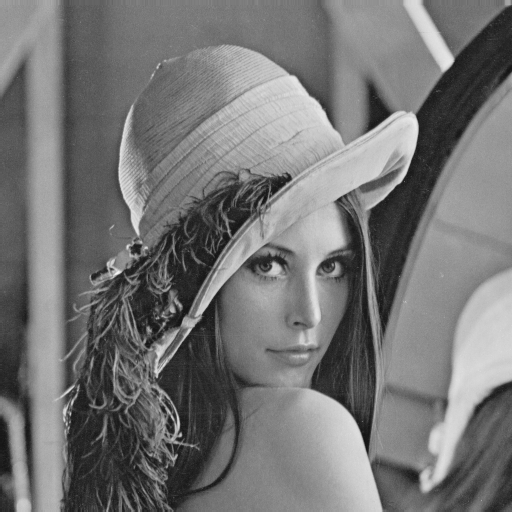
\includegraphics{Lenna.png} 
     \end{center} 

\begin{itemize}
\tightlist
\item
   Busque comandos para generar la matriz \(A\) asociada a esta imagen
  tal que los elementos esten en formato doble del IEEE y en el
  intervalo \([0,1]\). Muestre la submatriz \[X = \begin{bmatrix} 
     a_{240,240} & \cdots & a_{240,289} \\
     \vdots & & \vdots \\
     a_{289,240} & & a_{289,289}
     \end{bmatrix}\] así como la imagen correspondiente a esta
  submatriz.
\end{itemize}

    \begin{itemize}
\tightlist
\item
   Busque un comando para calcular el rango de una matriz y uselo para
  hallar el rango de \(A\) y \(X\). 
\end{itemize}

    \begin{quote}
 ¿\(A\) es invertible? ¿\(X\) es invertible?
\end{quote}

    \begin{itemize}
\tightlist
\item
   Apile las columnas \(X_1,\dots,X_{50}\) de \(X\) en un vector
\end{itemize}

\(x= \begin{bmatrix} X_1 \\ \vdots \\ X_{50}\end{bmatrix}\) 

    \begin{itemize}
\tightlist
\item
   Escriba un programa que genere la matriz de Toeplitz \(T\) de tamaño
  \(m\times m\) dada por
  \[t_{i,j}=\dfrac{1}{\sqrt{2\pi}\sigma}a^{(i-j)^2},\] donde
  \[a=\exp\left(\dfrac{-1}{2\sigma^2}\right)\] 
  \textbf{Entrada}:
  variables \(\sigma>0,m\in\mathbb N\) 
  
  \textbf{Salida}: arreglo \(T\) de
  \(m\times m\) que almacena matriz de Toeplitz 
  
  Evite realizar ciclos (for, while)
\end{itemize}

    \begin{itemize}
\tightlist
\item
  Fije \(m=2500\), 
  
  Para \(\sigma=0.5,1,1.5,1.8,2.0,2.5,3.0,3.5\) 
  \begin{itemize}
   \item[]  haga el producto \(y =Tx\) usando el programa anterior 
   \item[] Reacomode \(y\)
    como una matriz \(Y\) de tamaño \(50\times 50\) 
     \[Y = \begin{bmatrix}
          y_1 & y_{51} & \dots & y_{2491}\\ \vdots & \vdots & \vdots \\ 
          y_{50} & y_{100} & \dots & y_ {2500}\\
          \end{bmatrix}\] 
   \item[] Muestre la imagen correspondiente
  \end{itemize}
\end{itemize}


 \begin{quote}
 ¿cómo cambian las imágenes que obtiene en relación a la desviación
estándar \(\sigma\)?
\end{quote}

    \begin{itemize}
\tightlist
\item
   Fije \(m=2500\), genera una tabla con \(\text{cond}_1(T)\) para
  \(\sigma=1,1.5,1.8,2.0,2.1,2.3,2.5\) 
\end{itemize}

    \begin{quote}
 ¿qué puede decir del condicionamiento de \(T\) en relación a la
desviación estándar \(\sigma\)?
\end{quote}

    \begin{itemize}
\tightlist
\item
   En teoría, la matriz \(T\) es positiva definida para cualquier valor
  de \(\sigma>0\). Por lo que tiene factorización de Cholesky. 
  
  Sin embargo esto no es válido con el formato doble del IEEE. 
 
  Fije  \(m=50\). 
  
  \textbf{Halle al tanteo el valor más grande de \(\sigma>0\)}
  hasta con dos decimales (Ej. 3.56, 17.29) para el cúal pueda calcular
  la factorización de Cholesky de \(T\) 
\end{itemize}

    \begin{quote}
   use una rutina para la factorización de Cholesky 
 
   No es necesario mostrar las factorizaciones de Cholesky, pero sí el mensaje de error 
   de la rutina
\end{quote}

    \subsection{Ejercicio 5 (1.5 puntos)}\label{ejercicio-5}

 Halle un comando para generar la matriz de Hilbert \(H_n\) de tamaño
\(n\times n\).

\begin{itemize}
\tightlist
\item
   Construya una tabla que muestre \(\text{cond}_{\infty}(H_n)\) y
  \(\det(H_n)\) para \(n=1,\dots,30\) 
\end{itemize}

    \begin{quote}
¿cómo cambia el determinante conforme \(n\) aumenta?
\end{quote}

    \begin{itemize}
\tightlist
\item
   Gŕafique \(\text{cond}_{\infty}(H_n)\) contra \(n\) para
  \(n=1,\dots,30\) usando escala logarítmica para el eje vertical
\end{itemize}

    \begin{quote}
 ¿qué le dice la gráfica anterior sobre el condicionamiento de \(H_n\)?
\end{quote}

    \begin{itemize}
\tightlist
\item
   Sea \(u\) un vector de unos de \(n\) componentes. Sea \(b=Hu\).
  Calcule la solución \(\widehat x\) del sistema \(Hx=b\) mediante
  factorización LU con pivoteo por renglones y
  \(\|\widehat x-u\|_{\infty}\) para \(n=5,\dots,20\). 
\end{itemize}

\begin{quote}
\textbf{NOTAS}: 
 puede usar una rutina para factorización LU con pivoteo, 
 
 no muestre explicítamente todas las factorizaciones y las soluciones, 
 basta con la tabla de la normas \(\|\widehat x-u\|_{\infty}\)
\end{quote}

    \begin{quote}
 En teoría, \(\widehat x=u\). Por lo que
\(\|\widehat x-u\|_{\infty}=0\). ¿esto se refleja en los calculos que
hizo? ¿qué ocurre?
\end{quote}

    \subsection{Ejercicio 6 (2 puntos)}\label{ejercicio-6}

 Una manera de calcular los valores de la función \(u\) en el problema
de valores en la frontera \[\begin{array}{rl}
    -u''(x)+u(x) =1, & 0<x<1 \\ u(0)= 1, & \\ u(1) =0,  
    \end{array}\] es mediante el método de diferencias finitas. 
    
    Sea
\(h=\dfrac{1}{m+1}\)y sean \(x_j=jh\) para \(j=1,\dots,m\). 

Los valores
aproximados de \(u(x_j)\) son las componentes \(\widehat z_j\) de la
solución \(\widehat z\) del sistema de ecuaciones lineales \[Tz=b,\]
donde \[ T =
  \begin{bmatrix}
  2+h^2 & -1 & & 0 \\ -1 & \ddots & \ddots & \\ & \ddots & \ddots & -1 \\ 0 & & -1 & 2+h^2
  \end{bmatrix}\] es matriz tridiagonal simétrica \(m\times m\) y \[b=
\begin{bmatrix}
 h^2 +1 \\ h^2 \\ \vdots \\ h^2
\end{bmatrix}_{m\times 1}
\]\\

    \begin{itemize}
\tightlist
\item
   Busque una rutina para hallar la Factorización LU de una matriz
  tridiagonal simétrica y usela para resolver \(Tz=b\) cuando
  \(h=0.1,0.05,0.025,0.0125\) 
  \begin{itemize}
  \item[]  La rutina solo debe realizar operaciones con los elementos de la
   diagonal principal, la subdiagonal y la superdiagonal tanto en la
    Factorización como en las fases de sustitución directa y hacia átras.
  \end{itemize}
\end{itemize}


    \begin{itemize}
\tightlist
\item
   La función \[u(x)=1-\dfrac{\sinh(x)}{\sinh(1)}\] es la solución del
  problema de valores en frontera. 
  
  En una misma figura gráfique los
  valores \(u(x_j)\) contra \(x_j\) y las componentes \(\widehat z_j\)
  contra \(x_j\) para \(h=0.1\) 
\end{itemize}

    \begin{itemize}
\tightlist
\item
   Muestre una tabla con los errores \[\left\|
    \begin{bmatrix}
    u(x_1) \\ \vdots \\ u(x_m)
   \end{bmatrix} -
   \begin{bmatrix}
    \widehat z_1 \\ \vdots \\ \widehat z_m
   \end{bmatrix}
    \right\|_{\infty}\] para \(h=0.1,0.05,0.025,0.0125\) 
\end{itemize}


    % Add a bibliography block to the postdoc
    
    
    
    \end{document}
